%%%%%%%%%%%%%%%%%%%%%%%%%%%%%%%%%
% 					ACSD Thesis Template v.2018a				 		%
%%%%%%%%%%%%%%%%%%%%%%%%%%%%%%%%%
% HowTo: https://acsd.etit.tu-chemnitz.de:5001/doku.php?id=start (TBD)
%----------------------------------------------------------------------------------------
%	PACKAGES AND OTHER DOCUMENT CONFIGURATIONS
%----------------------------------------------------------------------------------------

\documentclass[oneside, paper=a4, fontsize=12pt, german, dissertation, open=right, colorpdf, dvipsnames]{scrreprt} 
% available options for this document class: 
% oneside/twoside: for one- or two-sided printing 
% english/german:
% dissertation: switches title page to dissertation style (submitted)
% final: works only in combination with "dissertation" option, switches titlepage style to final version (requires additional information)
% colorpdf: enebales full color mode (document will be greyscale if deleted - recommended for draft printing)

%%%%%%%%%%%%%%%%%%%%%%%%%%%%%%%%%%%%%%%%%
% Classicthesis Typographic Thesis
% Configuration File
%
% Important note:
% The main lines to change in this file are in the DOCUMENT VARIABLES
% section, the rest of the file is for advanced configuration.
%
%%%%%%%%%%%%%%%%%%%%%%%%%%%%%%%%%%%%%%%%%
%----------------------------------------------------------------------------------------
%	CHARACTER ENCODING
%----------------------------------------------------------------------------------------

\PassOptionsToPackage{utf8}{inputenc} % Set the encoding of your files. UTF-8 is the only sensible encoding nowadays. If you can't read äöüßáéçèê∂åëæƒÏ€ then change the encoding setting in your editor, not the line below. If your editor does not support utf8 use another editor!
\usepackage{inputenc}

\PassOptionsToPackage{listings, floatperchapter}{ACSDthesis}
% Available options: drafting parts manychapters floatperchapter listings

%----------------------------------------------------------------------------------------
%	USEFUL COMMANDS
%----------------------------------------------------------------------------------------

\newcommand{\ie}{i.\,e.}
\newcommand{\Ie}{I.\,e.}
\newcommand{\eg}{e.\,g.}
\newcommand{\Eg}{E.\,g.} 

\newcounter{dummy} % Necessary for correct hyperlinks (to index, bib, etc.)
\providecommand{\mLyX}{L\kern-.1667em\lower.25em\hbox{Y}\kern-.125emX\@}
\newlength{\abcd} % for ab..z string length calculation

%----------------------------------------------------------------------------------------
%	BIBLIOGRAPHY SETUP
%----------------------------------------------------------------------------------------

\usepackage{csquotes}
\PassOptionsToPackage{%
%backend=bibtex8, % Instead of bibtex
backend=biber,bibencoding=ascii,%
language=auto,%
style=numeric-comp,%
%%style=authoryear-comp, % Author 1999, 2010
%bibstyle=authoryear,dashed=false, % dashed: substitute rep. author with ---
sorting=nyt, % name, year, title
maxbibnames=10, % default: 3, et al.
%backref=true,%
natbib=true % natbib compatibility mode (\citep and \citet still work)
}{biblatex}
\usepackage{biblatex}

\DefineBibliographyStrings{english}{%
  mathesis = {Master's thesis},
}

\DefineBibliographyStrings{german}{%
  mathesis = {Masterarbeit},
  phdthesis = {Dissertation},
}

%----------------------------------------------------------------------------------------
%	PACKAGES
%----------------------------------------------------------------------------------------
 
%\PassOptionsToPackage{fleqn}{amsmath} % equations flushed left
\usepackage{amsmath, amsthm, amssymb, amsfonts} 
\DeclareMathOperator{\argmin}{argmin}

\PassOptionsToPackage{T1}{fontenc} % T2A for cyrillics
\usepackage{fontenc}
\usepackage{textcomp} % Fix warning with missing font shapes
\usepackage{scrhack} % Fix warnings when using KOMA with listings package  
\usepackage{xspace} % To get the spacing after macros right
\usepackage{mparhack} % To get marginpar right
\usepackage{fixltx2e} % Fixes some LaTeX stuff 
\PassOptionsToPackage{printonlyused, smaller}{acronym} % Include printonlyused in the first bracket to only show acronyms used in the text
\usepackage{acronym} % Nice macros for handling all acronyms in the thesis

\PassOptionsToPackage{pdftex}{graphicx}
\usepackage{graphicx} 
\usepackage{epsfig, epstopdf, tikz, calc}
\usepackage{enumerate, units, here}
\usepackage{multicol} % xcolor already loaded in style file
%\usepackage{todonotes}% um sich notizen zu machen wie z.b. dummie Bilder
%\usepackage{catchfile}
%\usepackage{autobreak} %kann in align umgebung seitenumbruch autom.

%----------------------------------------------------------------------------------------
%	FLOATS: TABLES, FIGURES AND CAPTIONS SETUP
%----------------------------------------------------------------------------------------

\usepackage{tabularx} % Better tables
\setlength{\extrarowheight}{3pt} % Increase table row height
\newcommand{\tableheadline}[1]{\multicolumn{1}{c}{\spacedlowsmallcaps{#1}}}
\newcommand{\myfloatalign}{\centering} % To be used with each float for alignment
\usepackage{caption}
\captionsetup{font=small, labelfont=bf}
\usepackage{subcaption}  

%----------------------------------------------------------------------------------------
%	CODE LISTINGS AND ALGOITHMS SETUP
%----------------------------------------------------------------------------------------

\usepackage{listings} 
%\lstset{emph={trueIndex,root},emphstyle=\color{BlueViolet}}%\underbar} % For special keywords
\lstset{language=[LaTeX]Tex,%C++ % Specify the language(s) for listings here
morekeywords={PassOptionsToPackage,selectlanguage},
keywordstyle=\color{RoyalBlue}, % Add \bfseries for bold
basicstyle=\small\ttfamily, % Makes listings a smaller font size and a different font
%identifierstyle=\color{NavyBlue}, % Color of text inside brackets
commentstyle=\color{BrickRed}\ttfamily, % Color of comments
stringstyle=\rmfamily, % Font type to use for strings
numbers=left, % Change left to none to remove line numbers
numberstyle=\scriptsize, % Font size of the line numbers
stepnumber=5, % Increment of line numbers
numbersep=8pt, % Distance of line numbers from code listing
showstringspaces=false, % Sets whether spaces in strings should appear underlined
breaklines=true, % Force the code to stay in the confines of the listing box
%frameround=ftff, % Uncomment for rounded frame
%frame=single, % Frame border - none/leftline/topline/bottomline/lines/single/shadowbox/L
belowcaptionskip=.75\baselineskip % Space after the "Listing #: Desciption" text and the listing box
}

\PassOptionsToPackage{linesnumbered, ruled}{algorithm2e}
\usepackage{algorithm2e}

%----------------------------------------------------------------------------------------

\usepackage{ACSDthesis} 

%----------------------------------------------------------------------------------------
%	USING DIFFERENT FONTS
%----------------------------------------------------------------------------------------

\usepackage[sfdefault]{roboto}
\usepackage{arev}

\newcommand{\bs}{\boldsymbol}
\newcommand{\bm}{\boldsymbol}

%\DeclareMathSizes{12}{11}{8.5}{7}
\linespread{1.1}
\setcapindent{1em}

%----------------------------------------------------------------------------------------
% RENEW DOTS
%----------------------------------------------------------------------------------------
\usepackage{accents}

\renewcommand*{\dot}[1]{%
  \begingroup
  \fontfamily{cmr}\selectfont{\accentset{\mbox{\bfseries\hspace{0.16ex}.}}{#1}}
  \endgroup
}

\renewcommand*{\ddot}[1]{%
  \begingroup
  \fontfamily{cmr}\selectfont{\accentset{\mbox{\bfseries\hspace{0.16ex}.\hspace{-0.25ex}.}}{#1}}
  \endgroup
}

%----------------------------------------------------------------------------------------
% USEFUL MAKROS
%----------------------------------------------------------------------------------------

\newcommand{\N}{\mathbb{N}}
\newcommand{\Z}{\mathbb{Z}}
\newcommand{\Q}{\mathbb{Q}}
\newcommand{\R}{\mathbb{R}}
\newcommand{\C}{\mathbb{C}}

 % Includes the file which contains all the document configurations and packages - make sure to edit this file

\addbibresource{thesis.bib} % The file housing your bibliography
%\addbibresource[label=ownpubs]{Self_Publications.bib} % Uncomment for optional self-publications

% Available Abbreviations: BA, MA, RP (Forschungsprojekt/Research Project) -> Dissertation is enabled via the ``dissertation'' option in documentclass (see above)
% The abbreviations are defined for both German and English
% You do not have to use the abbreviations but can enter the FULL thesis type manually 
\thesistype{MA} 
\usetikzlibrary{patterns}
\finaldate{May 4th 2018}

\title{A Template for Dissertations, Final Theses, and Research Projects} % Titel der Arbeit
\subtitle{May the force be with you.} % Untertitel (falls vorhanden)
\author{Felix Petzke} % Name des bearbeitenden Studenten

%%%%%%%% Specific information for option "dissertation" %%%%%%%%
\dateofbirth{29.08.1988} % Geburtstag des bearbeitenden Studenten
\placeofbirth{Magdeburg} % Geburtsort des bearbeitenden Studenten
%%%%%%%% Specific information for option "final" %%%%%%%% %%%%
\dateofsubmission{22.02.2022} 
\dateofdefence{33.03.3033} 
%%%%%%%%%%%%%%%%%%%%%%%%%%%%%%%%%%%%%%%

\supervisor{Dr.\,-Ing. Arne-Jens Hempel} % Betreuer #1
\supervisor{Prof. Charles Xavier (Firma X)} % Betreuer #2 (weitere Betreuer mit \supervisor{...} hinzufügen)

\examiner{Prof. Dr.\,-Ing. habil. Stefan Streif} % Prüfer (i.d.R. Prof. habil. Dr.\,-Ing. Stefan Streif); Für Dissertation: Gutachter (mehrere Gutachter möglich wie bei supervisor)

\company{Firma X} % (optional) Name der Firma; Logo in figures/company_logo.pdf

%\hyphenation{Put special hyphenation here}
\sloppy

\begin{document}

\frenchspacing % Reduces space after periods to make text more compact
\raggedbottom % Makes all pages the height of the text on that page

%----------------------------------------------------------------------------------------
%	PRE-CONTENT THESIS PAGES
%----------------------------------------------------------------------------------------

\pagenumbering{roman} % Roman page numbering prior to the start of the thesis content (i, ii, iii, etc)
\pagestyle{plain} % Suppress headers for the pre-content pages
\maketitle
\pagenumbering{Roman}

\setcounter{page}{1}
\pdfbookmark[1]{Kurzfassung}{Kurzfassung} % Bookmark name visible in a PDF viewer
\chapter*{\bfseries Kurzfassung} %mit * bedeutet, nicht im Inhaltsverzeichnis
\thispagestyle{empty}

kurze Zusammenfassung, tbd.

\cleardoublepage

\chapter*{\bfseries Abstract} %mit * bedeutet, nicht im Inhaltsverzeichnis
\thispagestyle{empty}

Short summary, tbd.

\cleardoublepage%%Abstract
% Table of Contents with respective options
\refstepcounter{dummy}
\pdfbookmark[1]{\contentsname}{tableofcontents} % Bookmark name visible in a PDF viewer
\setcounter{tocdepth}{2} % Depth of sections to include in the TOC - currently up to subsections
\setcounter{secnumdepth}{3} % Depth of sections to number in the text - currently up to subsubsections
\tableofcontents
\thispagestyle{empty}
\cleardoublepage % fix first bookmark after toc%%Inhaltsverzeichnis (including tocdepth & secnumdepth options)
\refstepcounter{dummy}
\addcontentsline{toc}{chapter}{Symbolverzeichnis}
%\pdfbookmark[1]{Symbolverzeichnis}{Symbolverzeichnis} % Bookmark name visible in a PDF viewer % not needed because its added to toc and therfore shows up as a bookmark

\allowdisplaybreaks
\chapter*{\bfseries Symbolverzeichnis}
\thispagestyle{empty}
\vspace{-.5em} % Fix Notation top margin! Do not edit or delete!!!
\begin{tabular}{@{} p{\figurelabelwidth} @{} p{\textwidth-\figurelabelwidth}}
$k$ 				 & time instant for the high level prediction model\\
$\kappa$ 			 & time instant for the low level prediction model\\
$\bm{x}$	  		 & state vector\\
$\bm{u}$		  	 & input vector\\
$\bm{y}$		  	 & output vector\\
$\bm{\bar{x}}$  	 & predicted state vector\\
$\bm{\bar{u}}$  	 & predicted input vector\\
$\bm{\bar{y}}$  	 & predicted output vector\\
$\bm{x}_{i}$	 	 & state vector of the $i^{\text{th}}$ subsystems\\
$\bm{u}_{i}$	 	 & input vector of the $i^{\text{th}}$ subsystems\\
$\bm{x}_{\max}$ 	 & upper bound for the state\\
$\bm{x}_{\min}$	 & lower bound for the state\\
$\bm{u}_{\max}$	 & upper bound for the input\\
$\bm{u}_{\min}$ 	 & lower bound for the input\\
$\bm{N}$	 	 	 & length of the prediction horizon\\
$\bm{I}$	 	 	 & identity matrix of appropriate dimension\\
$\mathcal{X}$	  	 & state sequence of the prediction\\
$\mathcal{U}$	 	 & input sequence of the prediction\\
$\mathbb{R}$	  	 & set of real numbers\\
$\mathbb{R}^{n}$& set of $n$-dimensional vectors of real numbers\\
$\mathbb{R}^{n \times m}$ & set of $n \times m$ matrices of real numbers\\
$\mathbb{U}$	  	 & set of feasible inputs\\
$\mathbb{X}$	  	 & set of feasible states\\
\end{tabular}                   
\cleardoublepage

%%Symbolverzeichnis
\refstepcounter{dummy}
\addcontentsline{toc}{chapter}{Abkürzungsverzeichnis}
%\pdfbookmark[1]{Abkürzungsverzeichnis}{Abkürzungsverzeichnis} % Bookmark name visible in a PDF viewer % not needed because its added to toc and therfore shows up as a bookmark

\begingroup 
\let\clearpage\relax
\let\cleardoublepage\relax
\let\cleardoublepage\relax

\chapter*{Abkürzungsverzeichnis}
\thispagestyle{empty}
\vspace{-.5em} % Fix LoA top margin! Do not edit or delete!!!
\begin{tabular}{@{} p{\figurelabelwidth} @{} p{\textwidth-\figurelabelwidth}}
\textbf{MPC} & Model Predicitive Control, modellprädiktive Regelung\\
\textbf{MPFC} & Model Predicitive Path Following Control, modellprädiktive Pfadfolgeregelung\\
\textbf{ACC} & Adaptive Cruise Control, Abstandsregeltempomat\\
\textbf{KPI} & Key Performance Indicator, Leistungskennzahl\\
\textbf{CI} & Continuous Integration, kontinuierliche Integration\\
\end{tabular}                
\endgroup
\cleardoublepage%%Symbolverzeichnis
\addtocontents{lof}{\protect\vspace{-.9em}} % Fix LoF top margin! Do not edit or delete!!!
\listoffigures\addcontentsline{toc}{chapter}{List of Figures}%%Abbildungsverzeichnis

\cleardoublepage
\pagestyle{scrheadings} % Show chapter titles as headings
\pagenumbering{arabic} % Arabic page numbering for thesis content (1, 2, 3, etc)
\cleardoublepage % Avoids problems with pdfbookmark
\renewcommand*{\arraystretch}{1}

%----------------------------------------------------------------------------------------
%	THESIS CONTENT - CHAPTERS
%----------------------------------------------------------------------------------------
\chapter{Introduction}
\thispagestyle{empty}

This chapter is an introduction to the topic of the thesis. It gives the reader an idea of the problem at hand and why it is relevant. Simplified pictures and illustrations help to understand the problem on a general level. 

\section{Packages}
This template already comes with a large variety of packages. \textsc{Before you add custom packages please check if they are not already included in} \texttt{ACSDthesis\_config.tex}\textsc{, since double inclusions can interfere with options and destroy the layout!} Table \ref{tab:packages} lists all included packages with their according options. If you need to add custom options for a specific package, use the \texttt{\textbackslash PassOptionsToPackage\{<options>\}\{<package>\}} command, \textsc{before} the package is included.
\begin{table}[H]
\centering
\caption{Packages included in this template. The entry \textit{cf. config} refers to the file \texttt{ACSDthesis\_config.tex}, where extended setups are included.}
\begin{tabular}{l | l || l | l || l | l}
Package			& Options 			& Package			& Options 			& Package			& Options 			\\ \hline
accents				&					&
acronym			& smaller			&
algorithm2e		&\textit{cf. config}	\\
amsmath			&					&
amsthm			&					&
amssymb			&					\\
amsfonts			&					&
babel				& ngerman	/english&
calc				&					\\
caption				&\textit{cf. config}	&
csquotes			&\textit{cf. config}	&
epsfig				&					\\
epstopdf			&					&
enumerate			&					&
fontenc				& T1				\\
fixltx2e				&					&
graphicx			& pdftex			&
here				&					\\
listings				&\textit{cf. config}	&
mparhack			&					&
multicol			&					\\
pdfpages			&					&
pstricks				&					&
scrhack				&					\\
subcaption			&					&
textcomp			&					&
tikz					&					\\
units				&					&
xcolor				& dvipsnames		&
xspace				&				
\end{tabular}
\label{tab:packages}
\end{table}

\section{Citation}
At some point in your thesis you will have to cite another author's work. If not you either did something extremely wrong or extremely right.\footnote{But probably the first of the two.} This template uses the \texttt{csquotes} package for citation, which is set up in the file \texttt{ACSDthesis\_config.tex}. In order to cite use the \texttt{\textbackslash cite\{<bibtexkey>\}} command. Natbib citation commands like \texttt{\textbackslash citet\{\}} are also supported. Table \ref{tab:citation} shows the different available commands and their results.

If you cite more than one paper at a time, \textsc{put them all in a comma-separated list within the same cite command!} For example, \texttt{\textbackslash cite\{Betti2013, Picasso2016\}} produces \cite{Betti2013, Picasso2016} and \texttt{\textbackslash cite\{Limon2008, Betti2013, Picasso2016\}} produces \cite{Limon2008, Betti2013, Picasso2016}.

\begin{table}[H]
\centering
\caption{Citation styles supported in this thesis using the bibtexkey \textit{Limon2008} as an example. If not otherwise specified by your supervisor, use the \texttt{\textbackslash cite\{<bibtexkey>\}} command.} 
\begin{tabular}{l | l }
Command & Result \\ \hline
\texttt{\textbackslash cite\{Limon2008\}}			& \cite{Limon2008}			\\
\texttt{\textbackslash cite[see][chap. 2]\{Limon2008\}} & \cite[see][chap. 2]{Limon2008} \\
\texttt{\textbackslash citet\{Limon2008\}}			& \citet{Limon2008}			\\
\texttt{\textbackslash citet*\{Limon2008\}}		& \citet*{Limon2008}		\\
\texttt{\textbackslash citeauthor\{Limon2008\}}	& \citeauthor{Limon2008}	\\
\texttt{\textbackslash citeyear\{Limon2008\}}		& \citeyear{Limon2008}	
\end{tabular}
\label{tab:citation}
\end{table}

\section{Block Diagrams and Code Snippets}
A small example of a simple block diagram in tikz is shown in Figure \ref{fig:simpletikz}. The according code is the following: 
\lstset{language=TeX} % HERE IS HOW TO INCLUDE SCOURCE CODE SNIPPETS IN YOUR TEXT
\begin{lstlisting}
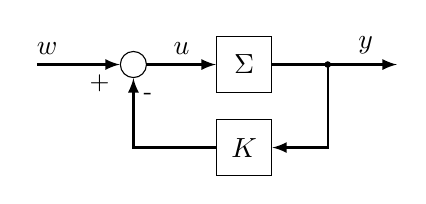
\begin{tikzpicture}
\tikzstyle{arrow} = [thick, color = black, -latex] % define standard arrow
\tikzstyle{block} = [draw, rectangle, minimum height = 2em, minimum width = 2em, align = center] % define standard block
\tikzstyle{dot} = [draw, shape = circle, inner sep = 0em, minimum size=0.15em, fill = black] % small dot on line junctions
\node(system)[block] at (0,0){$\Sigma$}; % draw system block at (0,0) -> reference for other stuff
\draw[arrow](system.east)--++(4.5em,0)node[near end, above]{$y$}; % draw output arrow of length 4em from sys block
\node(controller)[block, below of = system, node distance = 3em]{$K$}; % draw controller gain block
\draw[arrow](system.east)++(2em,0)node[dot]{}|-(controller.east); % draw arrow from output signal to controller gain
\node(sum)[draw, shape = circle, radius = 0.25em, left of = system, node distance = 4em]{}; % draw summation point
% draw arrows that connect with the summation point
\draw[arrow](controller.west)-|(sum.south)node[below right]{\small -}; % feedback
\draw[arrow](sum.west)++(-3em,0)--(sum.west)node[very near start, above]{$w$}node[below left]{\small +}; % reference
\draw[arrow](sum.east)--(system.west)node[midway, above]{$u$}; % input
\end{tikzpicture}
\end{lstlisting}

This was also an example of how to add code blocks to your text using the listings environment. The according setup is included in the file \texttt{ACSDthesis\_config.tex}. 

\begin{figure}
\centering
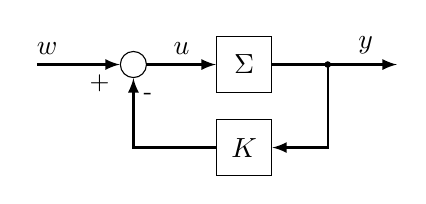
\begin{tikzpicture} % THIS IS A SIMPLE BLOCK DIAGRAM DONE IN TIKZ
\tikzstyle{arrow} 	= [thick, color = black, -latex] % define standard arrow
\tikzstyle{block} 	= [draw, rectangle, minimum height = 2em, minimum width = 2em, align=center] % define standard block
\tikzstyle{dot} 		= [draw, shape = circle, inner sep = 0em, minimum size=0.15em, fill=black] % small dot on line junctions

\node(system)[block] at (0,0){$\Sigma$}; % draw system block at (0,0) -> reference for other stuff
\draw[arrow](system.east)--++(4.5em,0)node[near end, above]{$y$}; % draw output arrow of length 4em from sys block
\node(controller)[block, below of = system, node distance = 3em]{$K$}; % draw controller gain block
\draw[arrow](system.east)++(2em,0)node[dot]{}|-(controller.east); % draw arrow from output signal to controller gain
\node(sum)[draw, shape = circle, radius = 0.25em, left of = system, node distance = 4em]{}; % draw summation point

% draw arrows that connect with the summation point
\draw[arrow](controller.west)-|(sum.south)node[below right]{\small -}; % feedback
\draw[arrow](sum.west)++(-3em,0)--(sum.west)node[very near start, above]{$w$}node[below left]{\small +}; % reference
\draw[arrow](sum.east)--(system.west)node[midway, above]{$u$}; % input
\end{tikzpicture}
\caption[Basic block diagrams in tikz]{This is an example for a simple block diagram using tikz.}
\label{fig:simpletikz}
\end{figure}

Note that it is often times a good idea to not write your tikz code directly in the source code, but to store it in a separate file and use the \texttt{\textbackslash input\{\}} command instead. This was for example done with Figure \ref{fig:problem}. 

\section{Definitions, Theorems, and so forth}
If you want to include definitions or theorems just use the respective environment, which are created with the usual \texttt{\textbackslash begin\{\}} and \texttt{\textbackslash end\{\}} commands. Available environments are \texttt{definition}, \texttt{assumption}, \texttt{lemma}, \texttt{theorem}, \texttt{proof}, and \texttt{remark}. It is of course also possible to reference them in the usual way.

\begin{definition}[Convexity]
A function $f:\mathcal{X}\to\mathcal{R}$ is called \textbf{convex}, if $\forall x, y\in\mathcal{X}, \forall t\in[0,1]:$ 
$f(tx+(1-t)y)\leq tf(x) + (1-t)f(y).$
\label{def:convexity}
\end{definition}
\begin{lemma}[Sum of convex functions]
Let $f:\mathcal{X}\to\mathcal{R}$ and $g:\mathcal{X}\to\mathcal{R}$ be two convex functions. Then the sum $h(x) = f(x)+g(x)$ is also convex.
\label{lem:sumconvex}
\end{lemma}
\begin{proof}[Proof of Lemma \ref{lem:sumconvex}]
The proof is trivial and follows directly from Definition \ref{def:convexity}. \qedhere
\end{proof}
\begin{remark}
Don't do proofs like that!
\end{remark}

\chapter{Problem Setup}
\thispagestyle{empty}
This chapter generally defines the actual problem to be addressed in this thesis. Illustrations help to explain the task to the reader.

\section{Simple Formulas and Complex Tikz}
Regarding this dummy thesis, a general hierarchical problem setup is depicted in Figure \ref{fig:problem}.\footnote{Just by chance it also gives you an example for a more complex block diagram using tikz.} The system $\bar{\mathcal{S}}$ used in the presented figure is defined as
\begin{align*}
\bar{\mathcal{S}}:
\begin{cases}
\dot{\bar{x}}=\bar{A}\bar{x}+\bar{B}\bar{u},\\
\bar{y}=\bar{C}\bar{x},
\end{cases}
\end{align*}
where $\bar{B}=\sum_{i=1}^{N}\hat{B}_{i}\alpha_{i}$. Is this was an actual thesis you should properly define all other variables that are used in a figure as well! But since this is a dummy, let's just pretend this was the case here. An important thing to note is that \LaTeX\; does not like footnotes and figures on the same page, since both take up space at the bottom.

The following section provides some dummy equations that utilize some nice alignments and combined equation numbering.

\begin{figure}
\centering
\rotatebox{90}{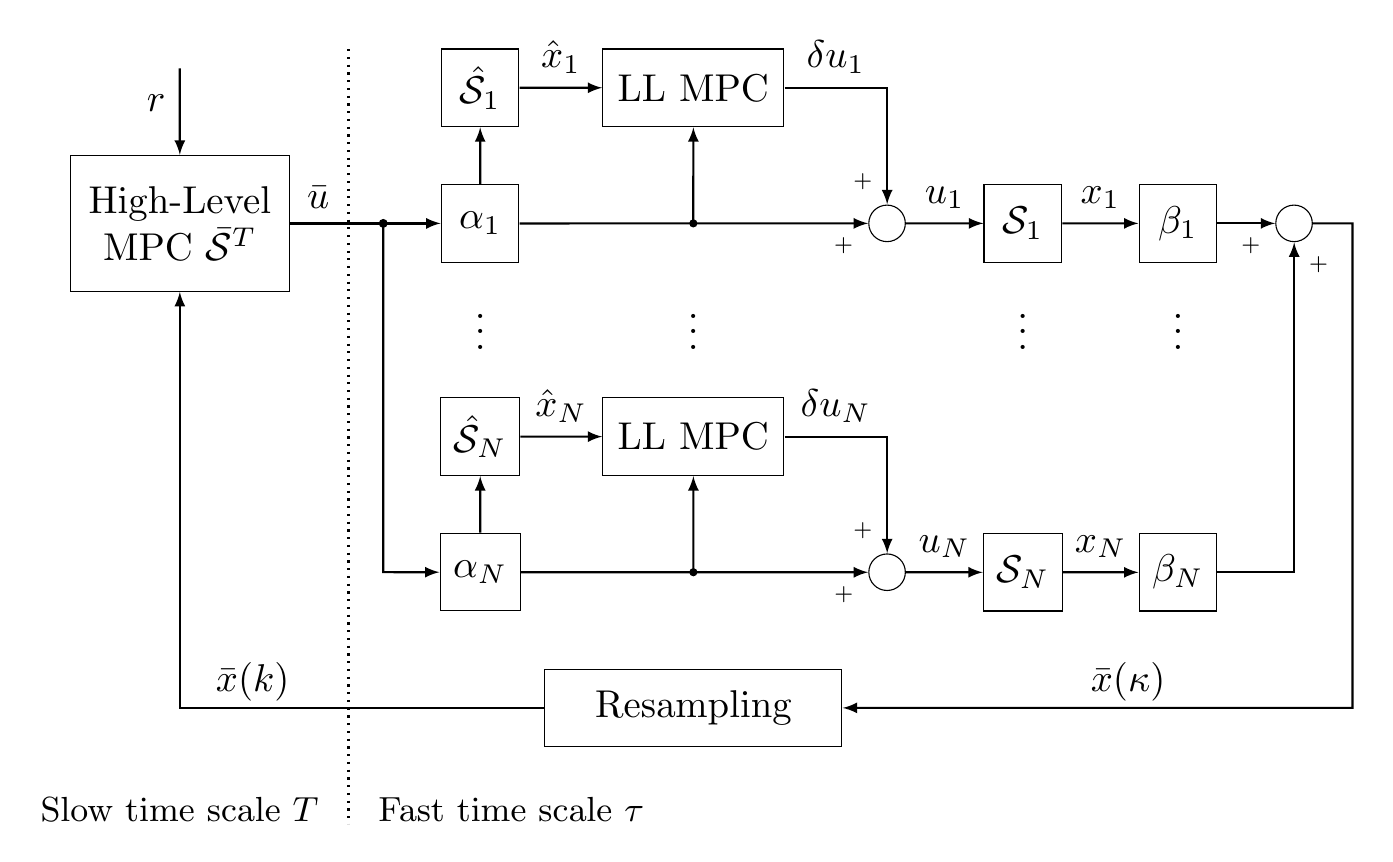
\begin{tikzpicture}[scale=1.4, every node/.style={scale=1.4}] 
% scale everything by factor 1.4 ^

\tikzstyle{sc} 		= [color = black] % shortcut for setting color to black
\tikzstyle{arrow} 	= [thick, color = black, -latex] % define standard arrow
\tikzstyle{sum} 	= [draw, shape = circle] % define summation symbol
\tikzstyle{dot} 		= [draw, shape = circle, inner sep = 0em, minimum size=0.15em, fill=black]
\tikzstyle{block} 	= [draw, rectangle, minimum height = 2em, minimum width = 2em] % define block
\tikzstyle{LLbox}	= [draw, rectangle, minimum height = 2em, minimum width = 4em, text width = 4em, align = center]

% define origin and High-Level MPC block with arrow
\node(tmp)[] at (0,0){}; 
\node(uRef)[block, minimum width=5em, minimum height=3.5em, text width=5em, align=center] at (0,0){High-Level MPC $\bar{\mathcal{S}}^{T}$};
\draw[arrow](uRef)++(0,4em)--(uRef) node[pos=0.4, left]{$r$};

% define auxiliary nodes
\node(aux1)[dot,minimum size=0.2em,right of=uRef, node distance=5.25em]{};
\node(auxN)[below of=aux1, node distance=9em]{};

% individual gains \alpha
\node(a1)[block,sc,right of=aux1,node distance=2.5em]{$\alpha_{1}$};
\node(aN)[block,sc,right of=auxN,node distance=2.5em]{$\alpha_{N}$};

% low level reference blocks
\node(r1)[block,sc,above of=a1,node distance=3.5em]{$\hat{\mathcal{S}}_{1}$};
\node(rN)[block,sc,above of=aN,node distance=3.5em]{$\hat{\mathcal{S}}_{N}$};

% LL MPC blocks
\node(l1)[LLbox,sc,right of=r1,node distance=5.5em]{LL MPC};
\node(lN)[LLbox,sc,right of=rN,node distance=5.5em]{LL MPC};

% summations
\node(s1)[sum,sc,right of=l1, node distance=5em, yshift=-3.5em]{};
\node(sN)[sum,sc,right of=lN, node distance=5em, yshift=-3.5em]{};

% arrows
\draw[arrow](l1)++(0,-3.5em)node[dot]{}--(l1);
\draw[arrow](lN)++(0,-3.5em)node[dot]{}--(lN);

\draw[arrow](a1)--(s1.west)node[below left]{\tiny +};
\draw[arrow](aN)--(sN.west)node[below left]{\tiny +};

\draw[arrow](l1.east)-|(s1.north)node[near start, above]{$\delta u_{1}$}node[above left]{\tiny +};
\draw[arrow](lN.east)-|(sN.north)node[near start, above]{$\delta u_{N}$}node[above left]{\tiny +};

\draw[arrow](a1)--(r1);
\draw[arrow](aN)--(rN);

\draw[arrow](r1)--(l1)node[midway, above]{$\hat{x}_{1}$};
\draw[arrow](rN)--(lN)node[midway, above]{$\hat{x}_{N}$};

\draw[arrow](uRef.east)--(aux1.center)node[pos=0.3, above]{$\bar{u}$}--(a1.west);
\draw[arrow](aux1.center)--(auxN.center)--(aN.west);

% real system blocks
\node(sys1)[block, right of=s1, node distance=3.5em]{$\mathcal{S}_{1}$};
\draw[arrow](s1.east)--(sys1.west) node[midway, above]{$u_{1}$};
\node(sysN)[block, right of=sN, node distance=3.5em]{$\mathcal{S}_{N}$};
\draw[arrow](sN)--(sysN) node[midway, above]{$u_{N}$};

% beta blocks with arrows
\node(b1)[block, right of=sys1, node distance=4em]{$\beta_{1}$};
\draw[arrow](sys1.east)--(b1.west) node[midway, above]{$x_{1}$};
\node(bN)[block, right of=sysN, node distance=4em]{$\beta_{N}$};
\draw[arrow](sysN)--(bN) node[midway, above]{$x_{N}$};

% sum before feedback with arrows
\node(srb)[sum,sc,right of=sys1, node distance=7em]{};
\draw[arrow](b1.east)--(srb.west) node[below left]{\tiny +};
\draw[arrow](bN.east)-|(srb.south) node[below right]{\tiny +};

% dots
\node[sc, below of=a1, node distance=2.5em]{$\vdots$};
\node[sc, below of=a1, node distance=2.5em, xshift=5.5em]{$\vdots$};
\node[sc, below of=sys1, node distance=2.5em]{$\vdots$};
\node[sc, below of=b1, node distance=2.5em]{$\vdots$};

% resampling block with arrows
\node(smp)[block, sc, below of=lN, node distance=7em, minimum width=7em, minimum height=2em, text width=7em, align = center]{Resampling};
\node(tmp1)[right of=srb, node distance=1.5em]{};
\draw[arrow](srb)--(tmp1.center)|-(smp.east)
	node[pos=0.72, above, yshift=-0.2em]{$\bar{x}(\kappa)$};
\draw[arrow](smp.west)-|(uRef.south)
	node[pos=0.4, above, yshift=-0.2em]{$\bar{x}(k)$};

% time scale separation
\draw[thick,dotted](uRef.east)++(1.5em,4.5em)--++(0em,-20em)
	node[left, anchor=south east, xshift=-0.4em, yshift=-0.3em]{\small Slow time scale $T$}
	node[right, anchor=south west, xshift=0.4em, yshift=-0.3em]{\small Fast time scale $\tau$};
\end{tikzpicture}
}
\caption[Complex block diagrams in tikz]{General problem setup. This is also an example for a more complex block diagram using tikz. The code for this picture is located in the separate file \texttt{./figures/tikz\_problem.tex}; it also demonstrates how to scale entire tikz-images. The last thing this figure shows is how to rotate things that are not images using the \texttt{\textbackslash rotatebox\{<angle>\}\{<stuff to rotate>\}} command. Since no positioning of the figure has been enforced, it got moved to the next page to avoid clashes with footnote 1.}
\label{fig:problem}
\end{figure}

\section{Formula Heaven}
The value function considered in the high-level MPC is defined as (cf. \cite{Betti2013})
\begin{align}
\begin{split}
V_{H}=&\;\|r-\bar{r}_{t}\|^{2}_{S}+\|\Delta\bar{x}(t+N_{H})\|^{2}_{P}+\|\bar{y}(t+N_{H})-\bar{r}_{t}\|^{2}_{P}\\&
+\sum_{k=t}^{t+N_{H}-1}\left\{\|\Delta\bar{x}(k)\|^{2}_{Q}+\|\bar{y}(k)-\bar{r}_{t}\|^{2}_{Q}+\|\Delta\bar{u}(k)\|^{2}_{R}\right\}.
\end{split}
\end{align}
The resulting optimization problem is then given by
\begin{align}
\begin{split}
\bar{u}^{\star} = &\;\arg\underset{\bar{u}, r_{t}}{\min}\left\{V_{H}(\delta\bar{x}_{t}, \bar{y}_{t}, r_{t}, \delta\bar{u}_{[t:t+N_{H}-1]}; x_{t}, y_{t}, r)\right\}\\
\text{s.t.}\;&\;\bar{\mathcal{S}}^{T},\\
&\;\delta\bar{u}(k)=\bar{u}(k)-\bar{u}(k-1)\\
&\;\bar{u}(k)\in\bar{\mathcal{U}}\\
&\;\bar{x}(k)\oplus\mathcal{W}\in\bar{\mathcal{X}}.
\end{split}
\end{align}
Always make sure to format your formulas in a pleasing way.



\chapter{Implementation}
\thispagestyle{empty}
The actual implementation of McNaughton's wrap around rule in MATLAB is done according to Algorithm \ref{alg:matlab}. This is also an example of how to incorporate algorithms in a beautiful way using the \texttt{algorithm} environment. If you want to customize the appearance of your algorithm, set it up in \texttt{ACSDthesis\_config.tex}. 

\begin{algorithm}[h]
\SetKwInOut{Input}{Input}
\SetKwInOut{Output}{Output}
\Input{$\left\{w_{ij}^q[\mu]\in[0,1] \;|\; j \in J, q\in Q\right\}$}
\For{$j = 1,\ldots, j_{\mathrm{max}}$}{ % for j
	\For{$q = 1,\ldots, q_{\mathrm{max}}$}{ % for q
		\eIf{$j=\;1\text{ and}\; q=1$} % if 1
		{$\eta_{11}^q[\mu] \leftarrow w_{11}^q[\mu]$} % then 1
		{\eIf{$q=1$} % else 1 start, if 2
			{$q_{-} \leftarrow q_{\mathrm{max}}$\\$j_{-} \leftarrow j-1$} % then 2
			{$q_{-} \leftarrow q-1$\\$j_{-} \leftarrow j$} % else 2
		$\sigma_{ij}^{q}[\mu] \leftarrow \eta_{ij_{-}}^{q_{-}}[\mu]$\\ % still else 1
		  \eIf { $\eta_{ij_{\mathrm{last}}}^{q_{-}}[\mu] + w_{ij}^q\le 1$} % if 3
			{$\eta_{ij}^{q}[\mu]\leftarrow\eta_{ij_{-}}^{q_{-}}[\mu]+w_{ij}^q[\mu]$} % then 3
			{$\eta_{ij}^{q}[\mu] \leftarrow  1$} % else 3
		} % else 1 end
	} % for j end
} % for q end
\Output{$\left\{(\sigma_{ij}^q[\mu],\eta_{ij}^q[\mu])\}\in [0,1]\times [0,1]\;|\;j\in J, q\in Q\right\}$}
\caption{McNaughton's wrap around algorithm.}
\label{alg:matlab}
\end{algorithm}











\chapter{Simulations}
\thispagestyle{empty}
This chapter is concerned with the results of the simulations and in particular with the inclusion of figures. Supported file formats are \texttt{.pdf}, \texttt{.eps}, \texttt{.jpg}, and \texttt{.png}. However, in order to achieve best results, try only to use vector graphics (\texttt{.pdf}/\texttt{.eps}) or high-resolution raster graphics (\texttt{.jpg}/\texttt{.png}).

\section{Single Figures and Cropping}
If you just want to include a single figure, use the \texttt{figure} environment together with the \texttt{\textbackslash includegraphics[<options>]\{<graphicpath>\}} command, where possible options are \texttt{width}, \texttt{height}, \texttt{scale}, and \texttt{angle}. Figure \ref{fig:trak}, for example, shows a nice picture of something technical. If you want to print out a draft version of your thesis without all the plots in order to save toner, you can also use \texttt{\textbackslash includegraphics[draft]\{<graphicpath>\}}, which replaces the figure by some empty space (cf. Fig. \ref{fig:draft}).

\begin{figure}
\centering
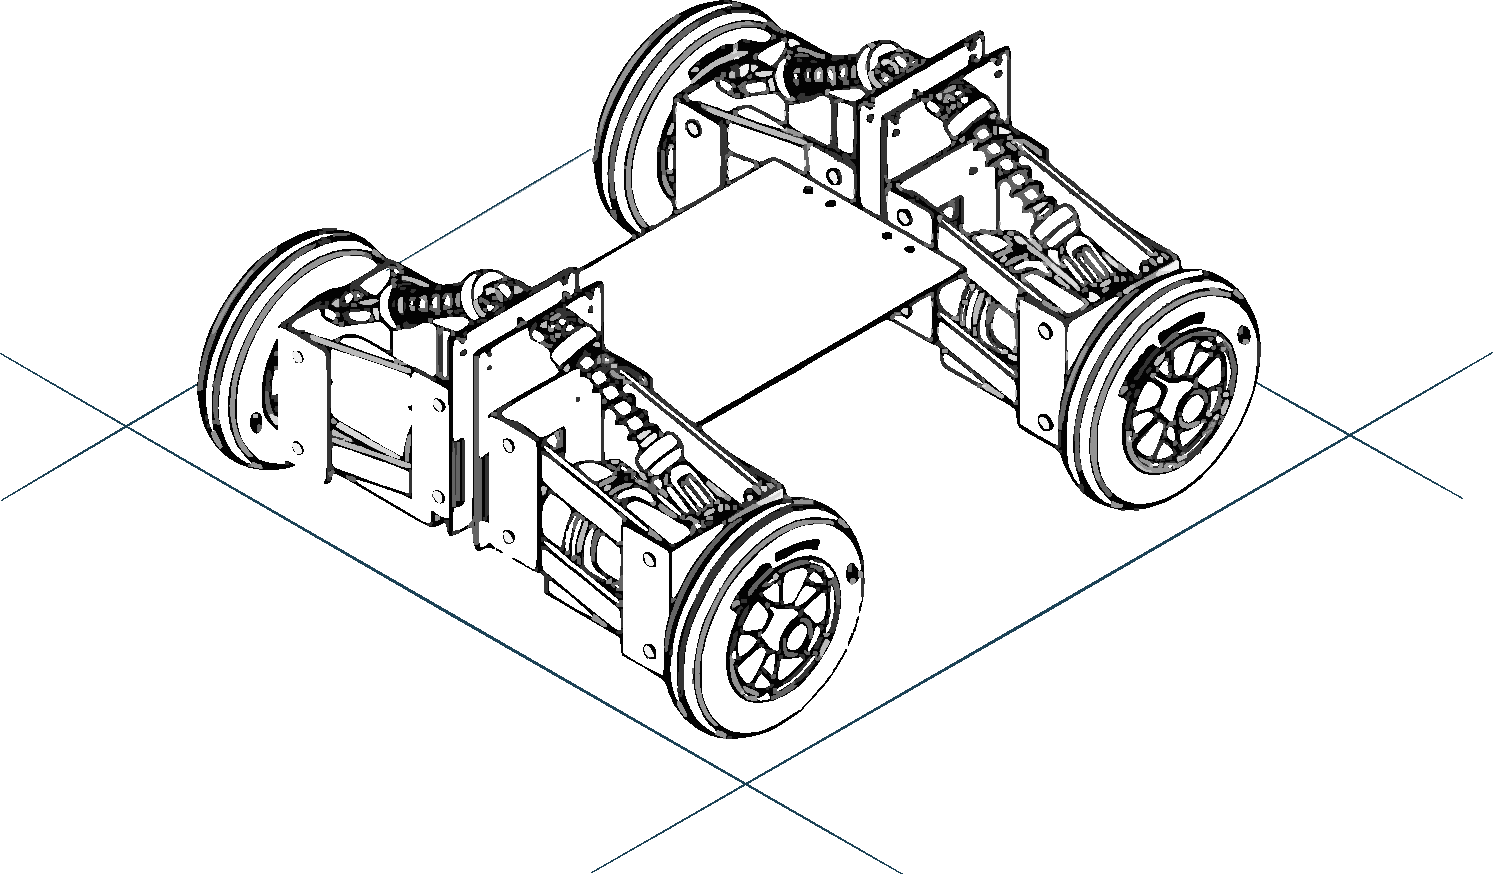
\includegraphics[width=0.5\textwidth]{figures/trak_skeleton}
\caption[Including an image with \texttt{\textbackslash includegraphics}]{A nice picture of something technical.}
\label{fig:trak}
\end{figure}

\section{Multi-Figures}
If you want to include several plots in one figure, use the \texttt{subfigure} environment within a \texttt{figure} environment. The subcaption package providing this environment is similar to subfig and subfigure, but comes with more flexibility and is a bit more intuitive. An example is given in Figure \ref{fig:options}, which also demonstrates the different options of the \texttt{\textbackslash includegraphics} command, like scaling, trimming, or rotating images. When you create a subfigure, make sure to use the \texttt{[b]} option which aligns the image on the bottom of its subfigure container: \texttt{\textbackslash begin\{subfigure\}\textbf{[b]}\{<widht>\}}. The necessary argument \texttt{<width>} specifies how big the ``containter'' for the image should be. 

Note that if the subcaptions of adjacent images span different numbers of lines they will not be aligned vertically (cf. Figs. \ref{fig:trim} and \ref{fig:smush} or Figs. \ref{fig:angle} and \ref{fig:draft}). In order to circumvent this issue you can use the alternative subcaption command \texttt{\textbackslash subcaptionbox[<list entry>]\{<heading>\}[<width>][<inner-pos>]\{<contents>\}} instead, which aligns captions at the top. An example is shown in Figure \ref{fig:capbox} -- compare the caption alignment of Figures \ref{fig:angle} and \ref{fig:draft} with Figures \ref{fig:angle2} and \ref{fig:draft2}.

\begin{figure}
\centering
\begin{subfigure}[b]{.3\linewidth}
	\centering
	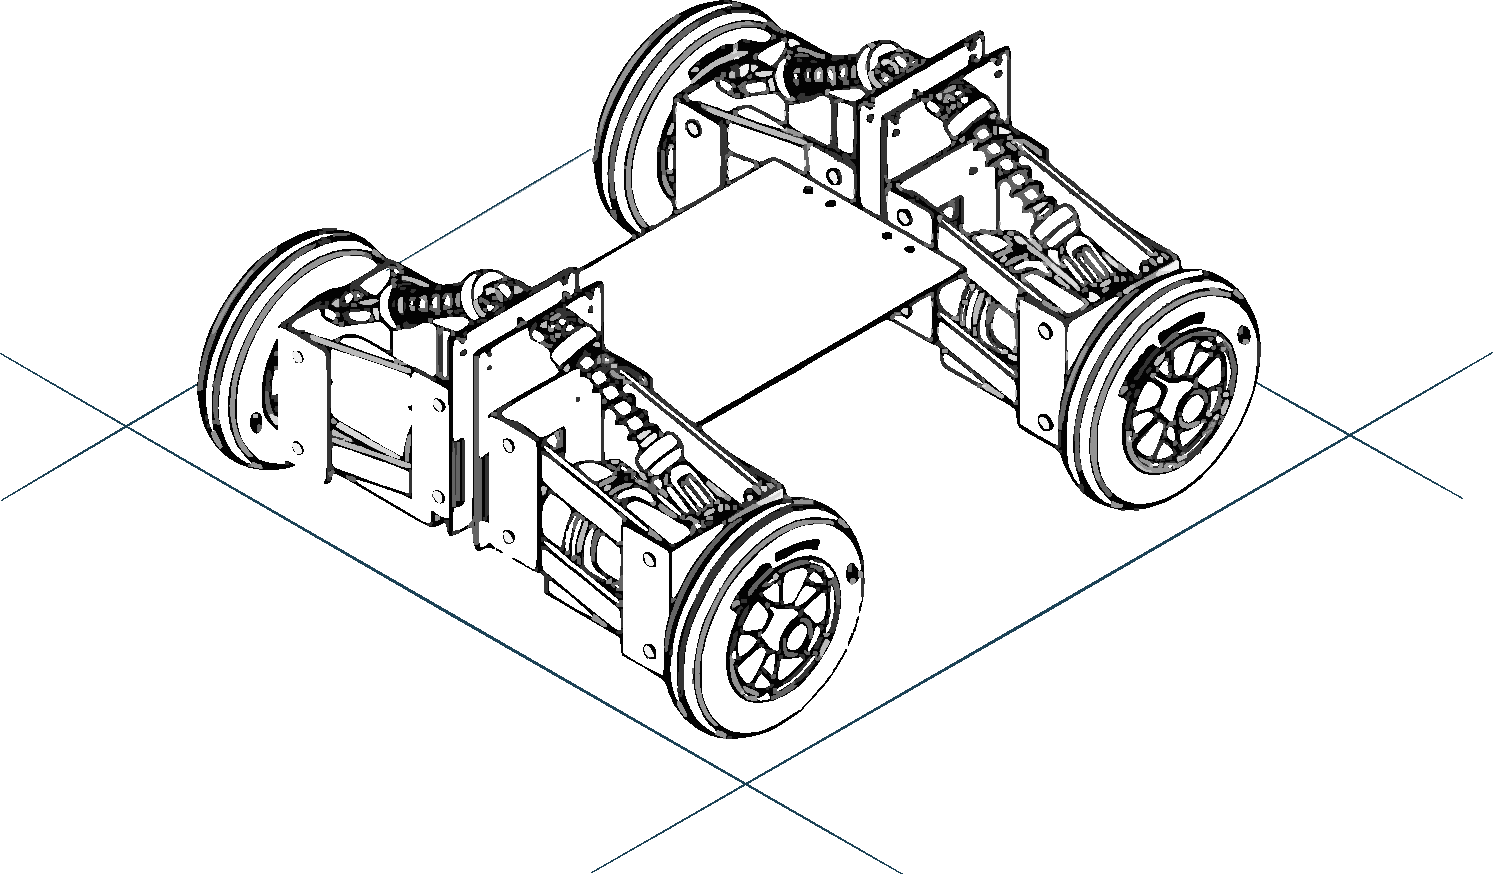
\includegraphics[scale=0.2,trim={3cm 2cm 4cm 0},clip]{figures/trak_skeleton}
	\caption{Options: scale=0.2, trim= \{3cm 2cm 4cm 0\}, clip.}
	\label{fig:trim}
\end{subfigure}\hfill
\begin{subfigure}[b]{.65\linewidth}
	\centering
	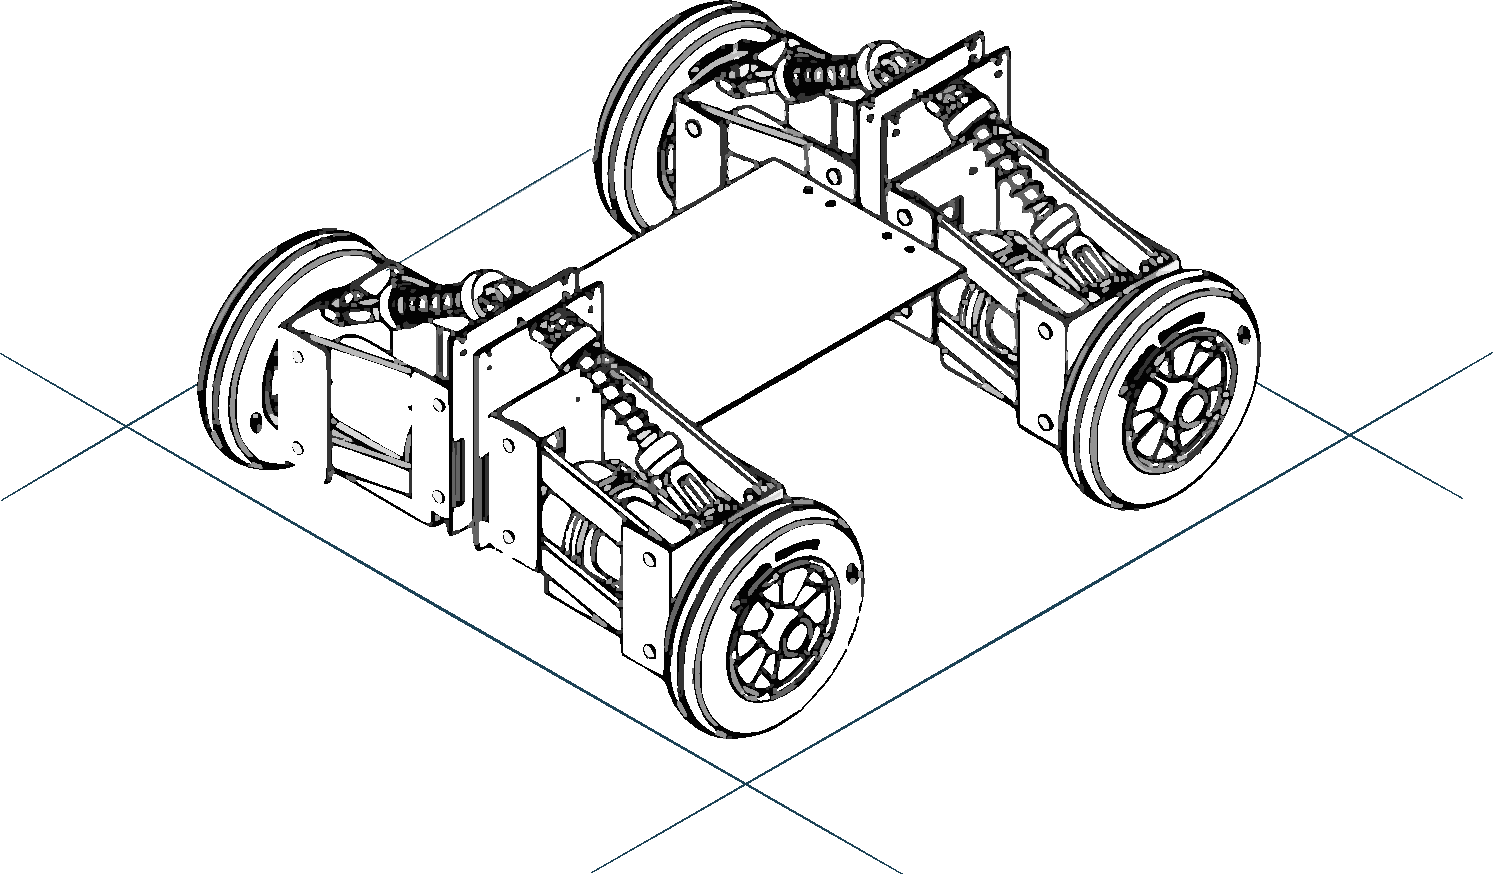
\includegraphics[width=\textwidth, height=2cm]{figures/trak_skeleton}
	\caption{Options: width=\textbackslash textwidth, height=2cm.}
	\label{fig:smush}
\end{subfigure}
\begin{subfigure}[b]{.45\linewidth}
	\centering
	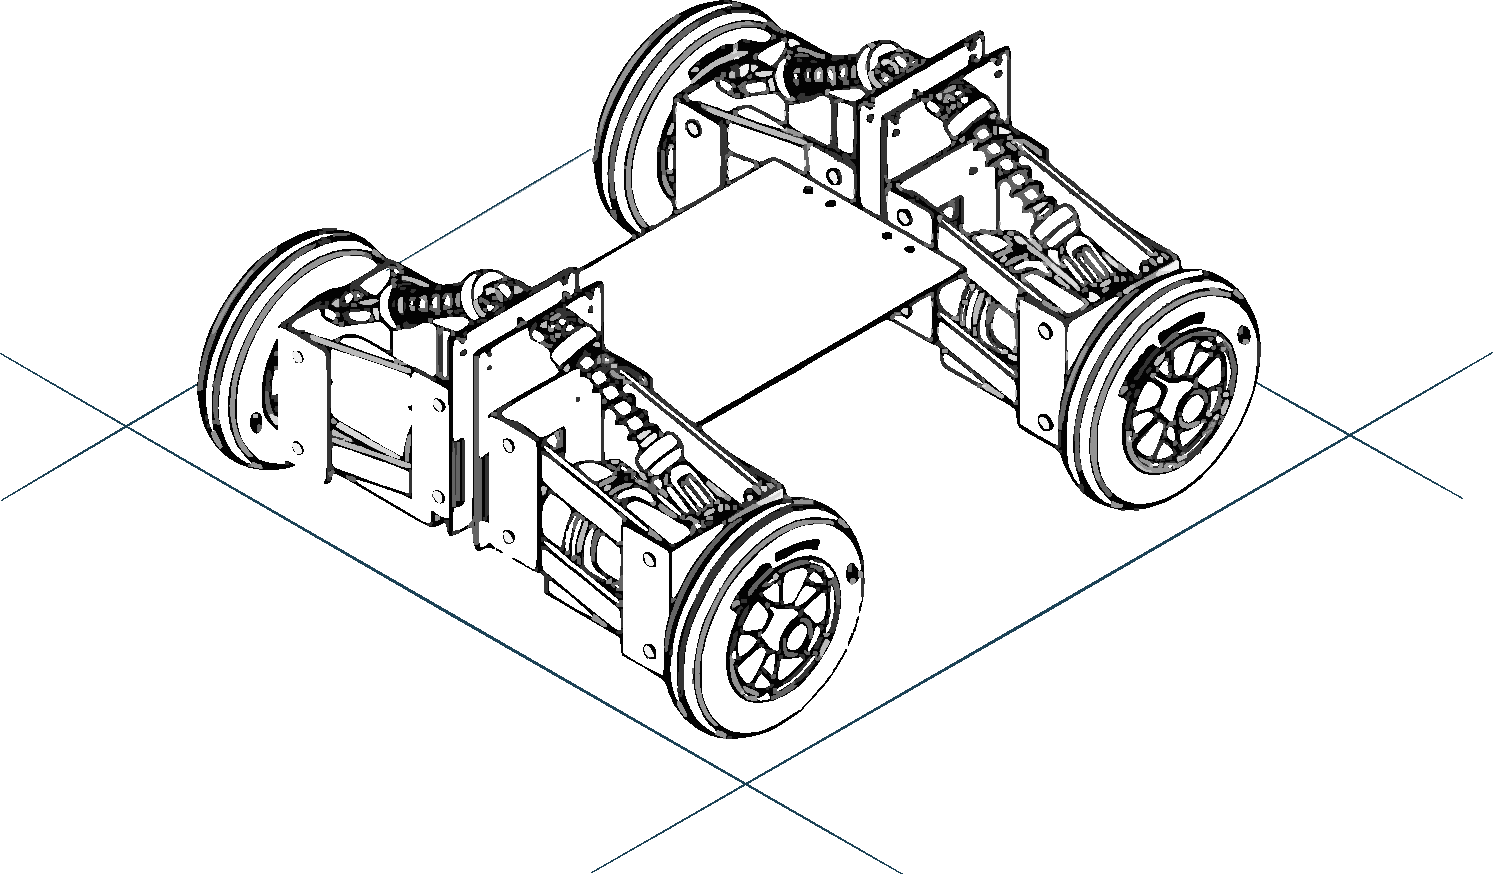
\includegraphics[width=5cm, angle=45]{figures/trak_skeleton}
	\caption{Options: width=5cm, angle=45.}
	\label{fig:angle}
\end{subfigure}\hfill
\begin{subfigure}[b]{.45\linewidth}
	\centering
	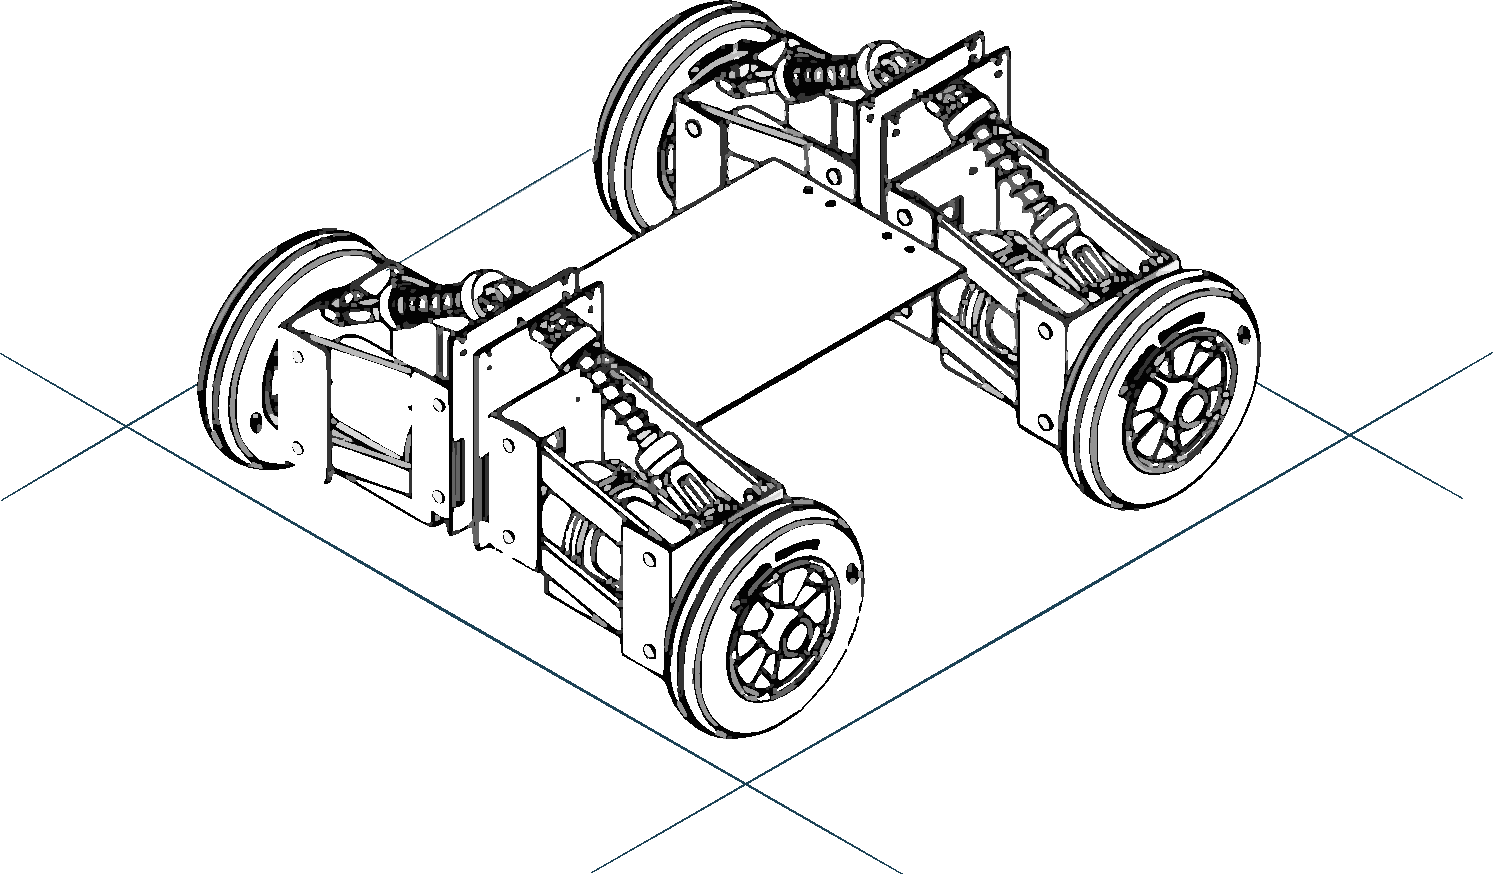
\includegraphics[draft, scale=0.25]{figures/trak_skeleton}
	\caption{Options: draft, scale=0.25. And this is some dummy text.}
	\label{fig:draft}
\end{subfigure}
\caption[Options of \texttt{\textbackslash includegraphics} and the \texttt{subfigure} environment]{Different options for the \texttt{\textbackslash includegraphics} command.}
\label{fig:options}
\end{figure}

\begin{figure}[H]
\centering
\subcaptionbox{Options: width=5cm, angle=45.\label{fig:angle2}}[.45\linewidth][c]{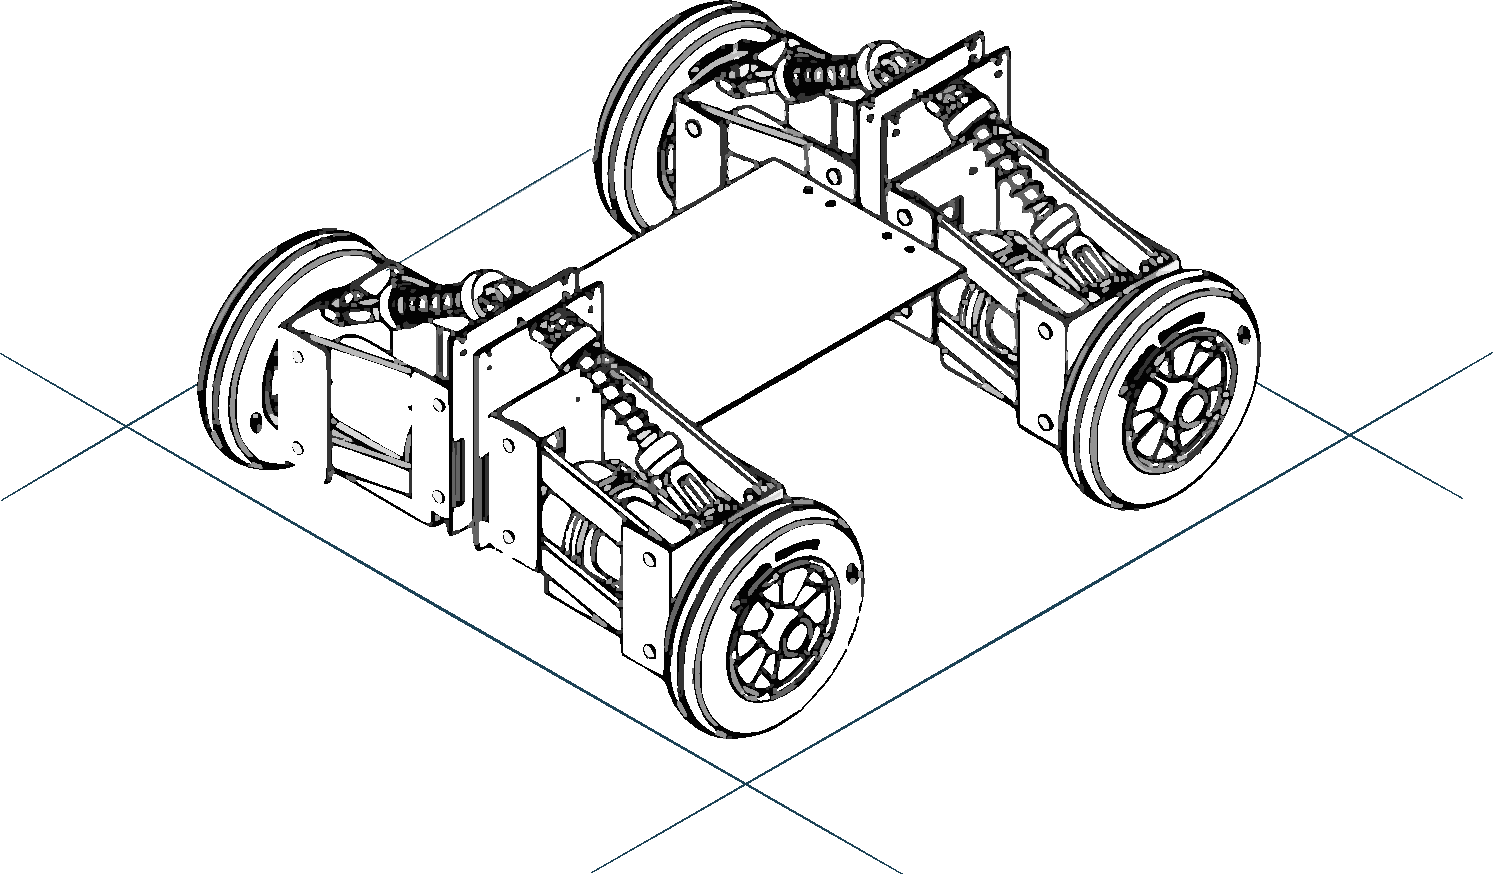
\includegraphics[width=5cm, angle=45]{figures/trak_skeleton}}
\hfill
\subcaptionbox{Options: draft, scale=0.25. And this is some dummy text.\label{fig:draft2}}[.45\linewidth][c]{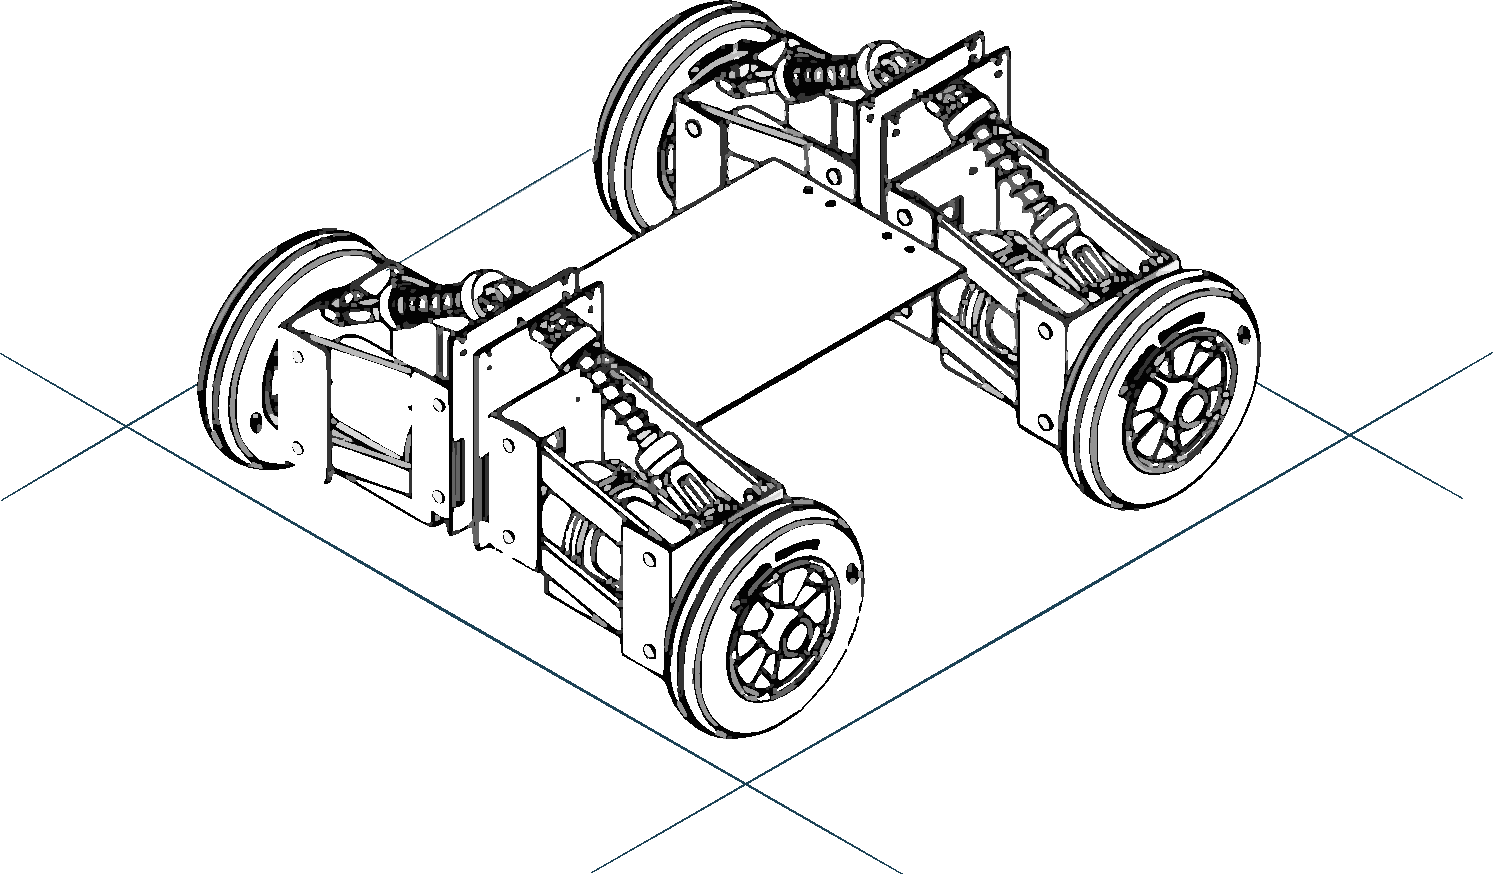
\includegraphics[draft, scale=0.25]{figures/trak_skeleton}}
\caption[\texttt{\textbackslash subcaptionbox} for multi-figures]{Effect of using \texttt{\textbackslash subcaptionbox}: All adjacent captions are aligned at the top, even if they span multiple lines.}
\label{fig:capbox}
\end{figure}



\chapter{Conclusion and outlook}
\thispagestyle{empty}
This template might still have some bugs or issues. If you encounter any, here is a checklist of what you should do:
\begin{enumerate}
\item \textsc{Download the latest version from our server!} I cannot stress this enough! You will find it either in \texttt{P:\textbackslash students\textbackslash common} or you can ask your supervisor.
\item Ask your fellow students if anyone has encountered the issue before and if they know what's the problem. 
\item Tell me (Felix Petzke) about the issue. I will then either provide you with a fix or a workaround. 
\end{enumerate}

Oh look, this was also an example for a numerated list using the \texttt{enumerate} environment. A list of bullet-points can be created with the \texttt{itemize} environment, as shown in the next section.

\section{Options of the ACSDthesis Package}
\label{sec:options}
You might ask why this section is almost at the end. As it turns out, most of the available options of the ACSDthesis package are not relevant during the writing process. Here is a list of available options and their respective effect:
\begin{itemize}
\item \texttt{onepage / twopage} -- toggle printing on one side or two sides (duplex). For optimal results with respect to the A5 book version (cf. Sec. \ref{sec:print}) only use the twopage option if you have more than 100 written pages of text in your PDF!
\item \texttt{english / german} -- toggle language setting. This will change all automatically generated marks and labels to the respective language.
\item \texttt{colorpdf} -- adding this will make all references colored. \textsc{Delete this option before creating your PDF for printing!} (cf. Section \ref{sec:print})
\item \texttt{parts} -- activate the \texttt{\textbackslash parts\{\}} command that is one layer above chapters. This option should only be used for very long theses and has to be passed to ACSDthesis in the file  \texttt{ACSDthesis\_config.tex}.
\end{itemize}

\section{Printing your Thesis}
\label{sec:print}
It is done! You finished your thesis! Now you just have to print it in our beautiful A5 book format so it can join its papery comrades in our ACSD library, to be read again by generations of suceeding students. 
The printing process is actually a piece of cake, thanks to our also available book cover template. The following steps will guide you to success:
\begin{enumerate}
\item Make sure that you typeset your thesis \textsc{without} the colorpdf option (cf. Sec. \ref{sec:options})! It will save you a \textsc{lot} of money!
\item Tell your supervisor that you are ready to print. He will have access to the cover template and help you with it.
\item If necessary, make sure you filled in all the information in the Statement of Authorship (Selbstst{\"a}ndigkeitserkl{\"a}rung) at that it has been properly attached to your thesis. You'll find it in the folder \texttt{99\_Authorship}.
\item Convert your thesis created with this template to an A5-version using the tex-file \texttt{MakeA5Version.tex}, which is contained in the folder of the cover-template.
\item Choose a cover image for your thesis and copy it to the cover template folder. This could be an illustration of the main method you used or just a nice picture that fits the topic of your thesis. However, make sure that there are no copyright issues!
\item Open up \texttt{MakeCover.tex} and fill in all the necessary data. Especially focus on
\begin{itemize}
\item the volume number of your thesis, which you will get from your supervisor;
\item the short title, which will be printed on the spine of the book and therefore has a limited length of about 70 letters (including whitespaces) -- this means that if your title has less than 70 letters you can use it as short title as well;
\item the number of \textit{printed} pages (\ie number of sheets of paper the printed thesis will have) at the very beginning of the code. Note that if you use two-sided printing the number of pages shown in the PDF editor is twice the number of printed pages! For optimal results this number should not be less than 50, so only use two-sided printing if you have more than 100 written pages!
\end{itemize}
\item Typeset the file and \textsc{check everything again on the produced PDF!} You can then tell Mr. Trompke that you are ready to print -- he will help you from here on.
\end{enumerate}




% Bibliography

\label{app:bibliography} % Reference the bibliography elsewhere with \autoref{app:bibliography}

\manualmark % Work-around to have small caps also here in the headline
\markboth{\spacedlowsmallcaps{\bibname}}{\spacedlowsmallcaps{\bibname}} % Work-around to have small caps also
%\phantomsection
\cleardoublepage % fix counter for next added section
\refstepcounter{dummy}

\addtocontents{toc}{\protect\vspace{\beforebibskip}} % Place the bibliography slightly below the rest of the document content in the table of contents
\addcontentsline{toc}{chapter}{\tocEntry{\bibname}}

\printbibliography


%----------------------------------------------------------------------------------------
%	STATEMENT OF AUTHORSHIP
%----------------------------------------------------------------------------------------
\cleardoublepage
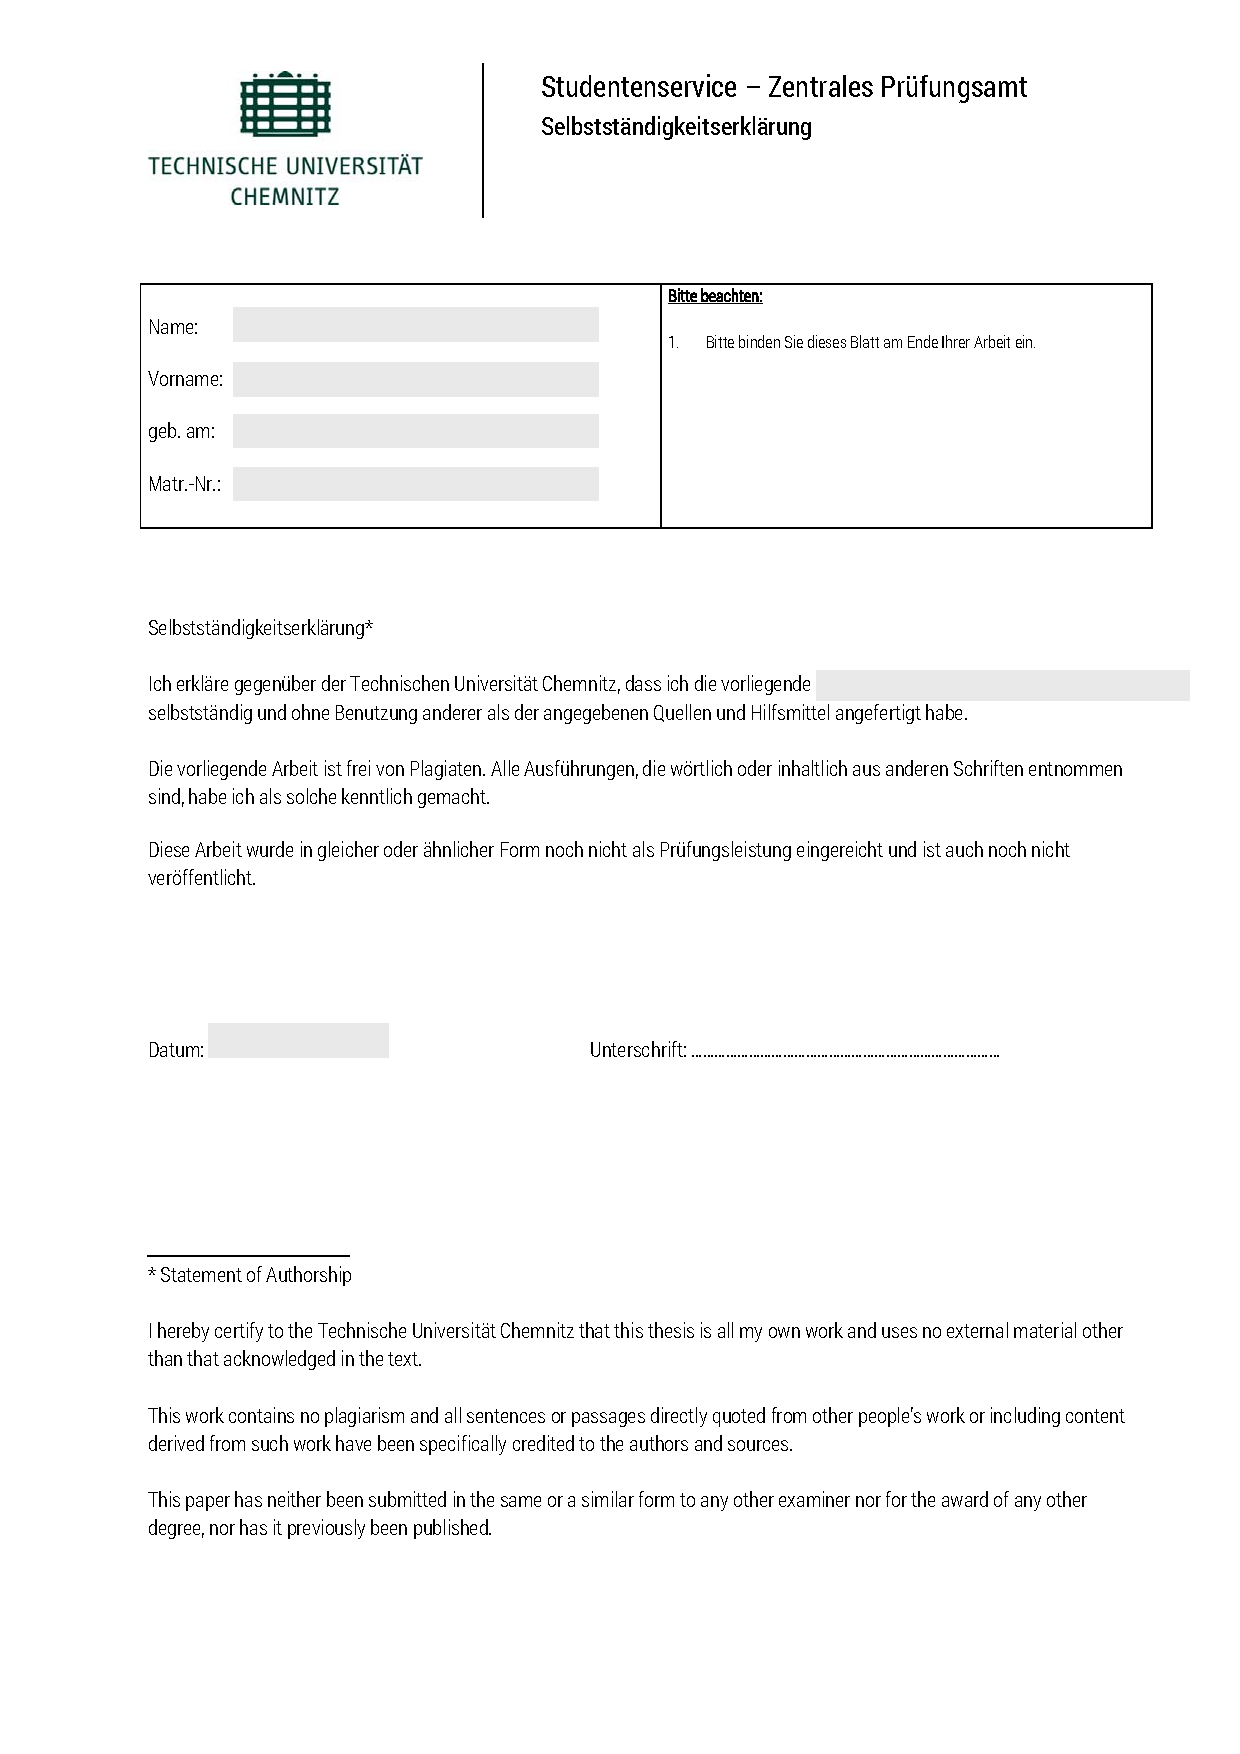
\includepdf[pages=-]{99_Authorship/selbststaendigkeitserklaerung} 
\cleardoublepage
\end{document}
